\subsection{Zadania}

\setcounter{problem}{0}

\begin{problem}
  Policja w Nowym Yorku próbuje złapać przestępce znajdującego się w punkcie $\otimes$. Obstawiła część ulic, ale nie wszystkie. Przestępca w każdym korku porusza się losowo (tzn. z prawdopodobieństwem $1/4$ w każdym z możliwych kierunków). Jeżeli wpadnie na policję $\bullet$ zostaje złapany, jeżeli dotrze do jednego z pól $\circ$ ucieka. Oblicz prawdopodobieństwo, że uda mu się uciec.

  \begin{center}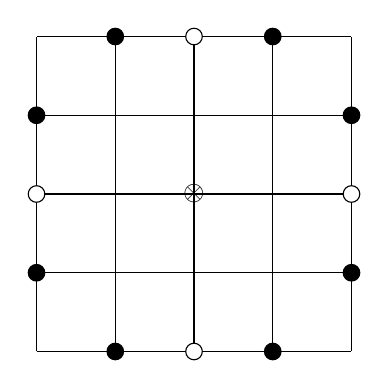
\begin{tikzpicture}
    \foreach \x in {0, ..., 4}
      {
        \draw(0,\x)--(4, \x);
        \draw(\x, 0)--(\x, 4);
      }

    \filldraw (0, 1) circle (3pt);
    \filldraw (0, 3) circle (3pt);
    \filldraw (1, 0) circle (3pt);
    \filldraw (3, 0) circle (3pt);
    \filldraw (3, 4) circle (3pt);
    \filldraw (1, 4) circle (3pt);
    \filldraw (4, 1) circle (3pt);
    \filldraw (4, 3) circle (3pt);
    \filldraw[fill=white] (0, 2) circle (3pt);
    \filldraw[fill=white] (4, 2) circle (3pt);
    \filldraw[fill=white] (2, 0) circle (3pt);
    \filldraw[fill=white] (2, 4) circle (3pt);

    \node at (2,2) {$\otimes$};
  \end{tikzpicture}\end{center}
\end{problem}

\begin{solution}
Zacznę od oznaczenia pozycji literkami:
\begin{center}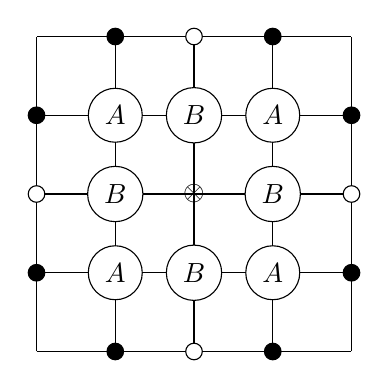
\begin{tikzpicture}[fun/.style={circle, color=black, fill=white, minimum size=3mm, draw=black, thin}]
    \foreach \x in {0, ..., 4}
      {
        \draw(0,\x)--(4, \x);
        \draw(\x, 0)--(\x, 4);
      }

    \filldraw (0, 1) circle (3pt);
    \filldraw (0, 3) circle (3pt);
    \filldraw (1, 0) circle (3pt);
    \filldraw (3, 0) circle (3pt);
    \filldraw (3, 4) circle (3pt);
    \filldraw (1, 4) circle (3pt);
    \filldraw (4, 1) circle (3pt);
    \filldraw (4, 3) circle (3pt);
    \filldraw[fill=white] (0, 2) circle (3pt);
    \filldraw[fill=white] (4, 2) circle (3pt);
    \filldraw[fill=white] (2, 0) circle (3pt);
    \filldraw[fill=white] (2, 4) circle (3pt);

    \node[fun] at (1, 1) {$A$};
    \node[fun] at (2, 1) {$B$};
    \node[fun] at (3, 1) {$A$};
    \node[fun] at (1, 2) {$B$};
    \node[fun] at (3, 2) {$B$};
    \node[fun] at (1, 3) {$A$};
    \node[fun] at (3, 3) {$A$};
    \node[fun] at (2, 3) {$B$};

    \node at (2,2) {$\otimes$};
  \end{tikzpicture}\end{center}
  oraz $\otimes$ jest oznaczone $S$, $\bullet$ to $0$ oraz $\circ$ będzie $1$. Niech $P_i$ oznacza prawdopodobieństwo ucieczki jeśli jesteśmy na polu $i$. Wtedy
  $$
    \begin{cases}
      P_S=\frac{1}{4}(P_B+P_B+P_B+P_B)=P_B\\ 
      P_B=\frac{1}{4}(P_1+P_S+P_A+P_A)=\frac{1}{4}(P_1+P_S)+\frac{1}{2}P_A\\ 
      P_A=\frac{1}{4}(P_B+P_B+P_0+P_0)=\frac{1}{2}(P_B+P_0)\\ 
      P_1=1\\ 
      P_0=0
    \end{cases}
  $$
  W takim razie $P_A=\frac{1}{2}P_B$ oraz
  $$
  P_B=\frac{1}{4}(1+P_S)+\frac{1}{4}P_B\implies 3P_B=1+P_S\implies 3P_B=1+P_B\implies P_B=\frac{1}{2}
  $$
  ale ponieważ $P_S=P_B$, to odpowiedź końcowa wynosi $\frac{1}{2}$.
\end{solution}

\begin{problem}
  Alicja i Robert rzucają symetryczną monetą tak długo aż wypadnie $OOOR$ lub $ORRR$. Alicja wygrywa, gdy wzorzec $OOOR$ wypadnie jako pierwszy, natomiast Robert, gdy wypadnie $ORRR$. Oblicz prawdopodobieństwo, że grę wygra Alicja.
\end{problem}

\begin{solution}
  Tak jak na wykładzie, rysujemy graf

\begin{center}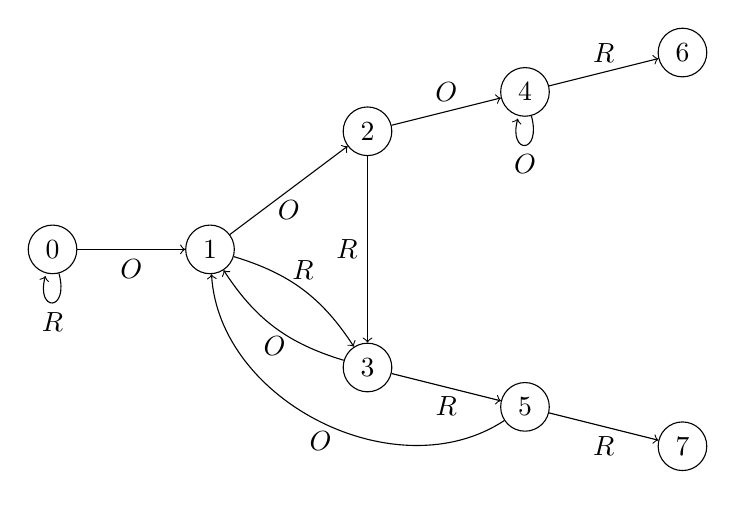
\begin{tikzpicture}[fun/.style={circle, draw=black, minimum size=1}]
  \node[fun] (s) at (0, 0) {$0$};
  
  \path (s) edge [loop below] node [midway, below] {$R$} (s);

  \node[fun] (o1) at (2, 0) {$1$};
  \path[->] (s) edge node [midway, below] {$O$} (o1);

  \node[fun] (o2) at (4, 1.5) {$2$};
  \path[->] (o1) edge node [midway, below] {$O$} (o2);

  \node[fun] (o3) at (4, -1.5) {$3$};
  \path[->] (o1) edge [bend left=20] node [midway, above] {$R$} (o3);
  \path[->] (o3) edge [bend left=20] node [midway, below] {$O$} (o1);
  \path[->] (o2) edge node [midway, left] {$R$} (o3);

  \node[fun] (o4) at (6, 2) {$4$};
  \path[->] (o2) edge node [midway, above] {$O$} (o4);
  \path[->] (o4) edge [loop below] node [midway, below] {$O$} (o4);

  \node[fun] (o5) at (6, -2) {$5$};
  \path[->] (o3) edge node [midway, below] {$R$} (o5);
  \path[->] (o5) edge [bend left=60] node [midway, below] {$O$} (o1);

  \node[fun] (o6) at (8, 2.5) {$6$};
  \path[->] (o4) edge node [midway, above] {$R$} (o6);

  \node[fun] (o7) at (8, -2.5) {$7$};
  \path[->] (o5) edge node [midway, below] {$R$} (o7);
  %\path[->] (o7) edge [bend left=80] node [midway, below] {$O$} (o1);

  \end{tikzpicture}\end{center}

  Alicja wygrywa w wierzchołku $6$ z $\prob$ $1$, a w wierzchołku $8$ wygrywa z $\prob$ równym $0$. Rozpisując to cudeńko jako równanie rekurencyjne, gdzie $P_i$ to prawdopodobieństwo, że będąc w wierzchołku $i$ wygra Alicja, dostajemy:
  $$
    \begin{cases}
      P_6=1\\ 
      P_8 = 0\\ 
      P_4 = \frac{1}{2} P_6 + \frac{1}{2} P_4 \\ 
      P_2 = \frac{1}{2} P_4 + \frac{1}{2} P_3 \\ 
      P_1 = \frac{1}{2} P_2 + \frac{1}{2} P_3 \\ 
      P_3 = \frac{1}{2} P_1 + \frac{1}{2} P_5 \\ 
      P_5 = \frac{1}{2} P_1 + \frac{1}{2} P_8
    \end{cases}
  $$

  Czyli $P_5=\frac{1}{2}P_1$, a 
  $$P_3=\frac{1}{2}P_1+\frac{1}{2}P_5=\frac{1}{2}P_1+\frac{1}{4}P_1=\frac{3}{4}P_1$$
  idąc z tym do $P_1$
  $$P_1=\frac{1}{2}P_2+\frac{1}{2}P_3=\frac{1}{2}P_2+\frac{3}{8}P_1$$
  z $P_4$ dostaniemy
  $$P_4=\frac{1}{2} P_6+\frac{1}{2}P_4=\frac{1}{2}+\frac{1}{2}P_4\implies \frac{1}{2}P_4=\frac{1}{2}\implies P_4=1$$
  i przechodzimy do $P_2$ na chwilę
  $$P_2=\frac{1}{2}P_4+\frac{1}{2}P_3=\frac{1}{2}+\frac{3}{8}P_1$$
  podstawiając z powrotem do $P_1$
  $$P_1=\frac{1}{2}P_2+\frac{3}{8}P_1=\frac{1}{4}+\frac{3}{16}P_1+\frac{6}{16}P_1=\frac{1}{4}+\frac{9}{16}P_1$$
  czyli $\frac{7}{16}P_1=\frac{1}{4}\implies P_1=\frac{4}{7}$, a ponieważ
  $$P_0=\frac{1}{2}P_0+\frac{1}{2}P_1\implies P_1=P_0$$
  to prawdopodobieństwo, że wygra Ala wynosi $\frac{4}{7}$.

\end{solution}

\begin{problem}
  Niech $\{\xi_k\}$ będzie ciągiem niezależnych zmiennych losowych z rozkładem $\prob{\xi_k=j}=p_j$. Pokaż, że $M_n=\max_{k\leq n}\xi_k$ jest łańcuchem Markowa. Jaka jest funkcja przejścia?
\end{problem}

\begin{solution}
  Chcemy pokazać, że
  $$\prob{M_{n+1}=m_{n+1}}{M_0=m_0,...,M_n=m_n}=\prob{M_{n+1}=m_{n+1}}{M_n=m_n}=P(m_n,m_{n+1})$$

  Zaczynamy od obserwacji, że $M_{n+1}=\max (\xi_{n+1},M_n)$ oraz, że $M_n\geq M_{n-1}\geq ...\geq M_0$. 
  \begin{align*}
    \prob{M_{n+1}=m_{n+1}}{M_0=m_0,...,M_n=m_n}&=\prob{M_{n+1}=\max(M_n, m_{n+1})}{M_0=m_0,...,M_n=m_n}=\\ 
                                               &=\prob{M_{n+1}=\max(M_n,m_{n+1})}{M_n=m_n}=P(m_n, m_{n+1})
  \end{align*}
  ponieważ $M_{n+1}=\max(M_n,m_{n+1})$, gdzie $m_{n+1}$ mamy ustalone odgórnie, jest zależne tylko od $M_n$.
  
  Wyrazem macierzy jest więc $P(m_n,m_{n+1})=\frac{p_{m_n}p_{m_{n+1}}}{p_{m_n}}=p_{m_{n+1}}$
\end{solution}

\begin{problem}
  Rozważmy łańcuch Markowa na przestrzeni stanów 
  $$S=\{s_1, s_2,s_3,s_4\}$$ 
  dla którego prawdopodobieństwa przejścia są zadane macierzą
  $$P=\begin{bmatrix}0 &\frac{1}{2} & \frac{1}{2} & 0\\ 
  0 & \frac{1}{3} &\frac{1}{3} & \frac{1}{3}\\ 
  0 & \frac{1}{3} & \frac{1}{3} & \frac{1}{3}\\ 
0 & \frac{1}{3} & \frac{1}{3} & \frac{1}{3}\end{bmatrix}$$
tzn. $\prob{X_{n+1}=s_j}{X_n=s_i}=P(i,j)$. Dla każdego stany oblicz $\lim_n \prob{X_n=s_i}{X_0=s_1}$.
\end{problem}

\begin{solution}
  Chyba można tutaj użyć kolejnego zadania.
\end{solution}

\begin{problem}
  Niech $\{X_n\}$ będzie łańcuchem Markowa o przeliczalnej przestrzeni stanów $S$ i macierzy przejścia $P$. Pokaż, że 
  \begin{enumerate}
    \item $\prob{X_n=x_n,X_{n-1}=x_{n-1},...,X_0=x_0}=\prob{X_0=x_0}P(x_0,x_1)...P(x_{n-1},x_n)$
    \item $\prob{X_{n+m}=y}{X_m=x}=\prob{X_n=y}{X_0=x}=P^n(x, y)$
    \item (Równanie Chapmana-Kolmogorowa)
      $$\prob{X_{n+m}=z}{X_0=x}=\sum_{y\in S}\prob{X_m=y}{X_0=x}\prob{X_n=z}{X_0=y}$$
  \end{enumerate}
\end{problem}

\begin{solution}
  \begin{enumerate}
    \item Może indukcją? Dla $n=0$ jest oczywiste, bo wtedy $\prob{X_0=x_0}=\prob{X_0=x_0}$ :v

      To teraz przejście $n\implies n+1$. Zacznę od czegoś co wiem, tzn. prawdopodobieństwa warunkowego
      \begin{align*}
        P(x_n, x_{n+1})=\prob{X_{n+1}=x_{n+1}}{X_n=x_n}&=\prob{X_{n+1}=x_{n+1}}{X_n=x_n,...,X_0=x_0}=\\ 
                                                       &=\frac{\prob{X_{n+1}=x_{n+1}, X_n=x_n,...,X_0=x_0}}{\prob{X_n=x_n,....,X_0=x_0}}
      \end{align*}

      No dobra, ale to co jest na dole to z założenia indukcyjnego wiemy, że 
      $$\prob{X_n=x_n,...,X_0=x_0}=\prob{X_0=x_0}P(x_0, x_1)...P(x_{n-1},x_n)$$
      podstawiając do tego równania wyżej dostajemy
      $$P(x_n,x_{n-1})=\frac{\prob{X_{n+1}=x_{n+1},...,X_0=x_0}}{\prob{X_0=x_0}P(x_0,x_1)...P(x_{n-1},x_n)}$$
      wystarczy przemnożyć i gotowe.
    \item Tutaj też chyba chcemy indukcję po $n$, a $m$ ustalamy stały?

      Base case to $n=0$ i wówczas
      $$\prob{X_{0+m}=y}{X_m=x}=\prob{X_0=y}{X_0=x}=P^0(x, y)=Id$$
      jest macierzą identyczności co ma sens - $X_m=y\;i\; X_m=x$ zachodzi z $\prob$ jeden jeśli $x=y$, a z $\prob=0$ jeśli są różne.

      To teraz $n\implies n+1$.

%      Zacznijmy od zapisania $P^{n+1}(x,y)$ zgodnie z definicją na wykładzie
%      \begin{align*}
%        P^{n+1}(x, y)&=\sum_{z\in S}P^n(x, z)P(z, y)=\sum_{z\in S}\prob{X_{n}=z}{X_0=x}P(z, y)=\\ 
%                     &=\sum_{z\in S}\frac{\prob{X_n=z,X_0=x}}{\prob{X_0=x}}P(z,y)=\\ 
%                     &=\sum_{z\in S}\frac{P(x, x_1)P(x_1, x_2)...P(x_{n-1}, z)P(z, y)}{\prob{X_n=z,X_{n-1}=x_{n-1},....,X_0=x}}\prob{X_n=z, X_0=x}=\\
%                     &=\sum_{z\in S}\frac{\prob{X_{n+1}=y,X_n=z,...,X_0=x}}{\prob{X_0=x}\prob{X_n=z,X_{n-1}=x_{n-1},...,X_0=x}}\prob{X_n=z,X_0=x}=\\ 
%                     &=\sum_{z\in S}\prob{X_{n+1}=y}{X_n=z}\prob{X_n=z}{X_0=x}=\\ 
%                     &=\sum_{z\in S}\frac{\prob{X_{n+1}=y, X_n=z}\prob{X_n=z,X_0=x}}{\prob{X_0=x}\prob{X_n=z}}
%      \end{align*}

      \begin{align*}
        \prob{X_{n+1}=y}{X_0=x}&=\frac{\prob{X_{n+1}=y, X_0=x}}{\prob{X_0=x}}=\\ 
                               &=\sum_{x_n\in S}\frac{\prob{X_{n+1}=y, X_0=x}}{\prob{X_n=x_n, X_0=x}} \frac{\prob{X_n=x_n, X_0=x}}{\prob{X_0=x}}=\\ 
                               &=\sum_{x_n\in S}\frac{\prob{X_{n+1}=y, X_0=x}}{\prob{X_n=x_n, X_0=x}}P^n(x, x_n)=\\ 
                               &=\sum_{z\in S}\frac{\prob{X_{n+1}=y}{X_0=x}}{\prob{X_n=z}{X_0=x}}P^n(x, z)
      \end{align*}
      a idąc od prawej strony dostalibyśmy, że
      \begin{align*}
        P^{n+1}(x, y)&=\sum_{z\in S}P^n(x, z)P(z, y)=\sum_{z\in S}P^n(x, z)\prob{X_{n+1}=y}{X_n=z}=\\ 
                     &=\sum_{z\in S}\frac{\prob{X_{n+1}=y, X_n=z}}{\prob{X_n=z}}P^n(x, z)
      \end{align*}

      \begin{align*}
        \prob{X_{n+1}=y, X_n=x_n,..., X_0=x}&=\prob{X_0=x, X_1=x_1}\frac{\prob{X_1=x_1, X_2=x_2}}{\prob{X_1=x_1}}...\frac{\prob{X_{n+1}=y, X_n=x_n}}{\prob{X_n=x_n}}
      \end{align*}

    \item To chyba pójdzie indukcją po $m$ korzystającą z poprzedniego punktu.

      \begin{align*}
        \prob{X_{n+m+1}=y}{X_0=x}&=P^{n+m+1}(x, y)=\sum_{z\in S}P^{n+m}(x, z)P(z, y)=\\ 
                                 &=\sum_{z\in S}\prob{X_{n+m}=z}{X_0=x}\prob{X_{n+1}=y}{X_n=z}=\\ 
                                 &=\sum_{z\in S}\sum_{s\in S}\prob{X_m=z}{X_0=x}\prob{X_n=s}{X_0=x}\prob{X_{n+1}=y}{X_n=z}=\\ 
                                 &=\sum_{z\in S}\prob{X_{n+1}=y}{X_n=z}\prob{X_n=z}{X_0=x}\sum_{s\in S}\prob{X_m=s}{X_0=x}=\\ 
                                 &=\sum_{z\in S}\prob{X_{n+1}=y}{X_n=z}\prob{X_n=z}{X_0=x}\sum_{s\in S}P^m(x, s)=\\ 
                                 &=\sum_{z\in S}\prob{X_{n+1}=y}{X_n=z}\prob{X_n=z}{X_0=x}\cdot 1
      \end{align*}
  \end{enumerate}
\end{solution}
